% answers.tex —— 2013 年·四川卷·文科 · 参考答案与详细解析片段
% 由 tools/generate_projects.py 依来源总账自 2013/2013_数学真题_四川文_试题.md + 2013/2013_数学真题_四川文_解析正文.md + 2013/2013_数学真题_四川文_答案要点.md 生成，勿手改（改源 MD 后重跑）

\begin{answer}
\gksolhead{1}{}

\textbf{题目}：

设集合 $A=\{1,2,3\}$，集合 $B=\{-2,2\}$，则 $A\cap B=$\mbox{（　　）}
（A）$\varnothing$；（B）$\{2\}$；（C）$\{-2,2\}$；（D）$\{-2,1,2,3\}$。

\Needspace{4\baselineskip}
\textbf{解析}
\Needspace{5\baselineskip}
$A=\{1,2,3\}$ 与 $B=\{-2,2\}$ 的公共元素只有 $2$，故
\nopagebreak[4]
\[A\cap B=\{2\}.\]
选 B。

\gkanswer{答案：B。}

\end{answer}
\begin{answer}
\gksolhead{2}{}

\textbf{题目}：

一个几何体的三视图如图所示，则该几何体可以是\mbox{（　　）}
\nopagebreak[4]
\begin{center}% 2013 四川卷文科第 2 题：几何体的三视图（正、侧视图为等腰梯形，俯视图为同心圆）。
\begin{tikzpicture}[font=\footnotesize, line width=0.45pt, scale=1]
  % 正视图：梯形
  \draw (0.35,0) -- (2.95,0) -- (2.20,1.55) -- (1.10,1.55) -- cycle;
  \node[below] at (1.65,-0.16) {正视图};
  % 侧视图：梯形
  \draw (4.55,0) -- (7.15,0) -- (6.40,1.55) -- (5.30,1.55) -- cycle;
  \node[below] at (5.85,-0.16) {侧视图};
  % 俯视图：同心圆
  \draw (1.65,-1.55) circle (0.90);
  \draw (1.65,-1.55) circle (0.46);
  \node[below] at (1.65,-2.62) {俯视图};
\end{tikzpicture}
\end{center}
\nopagebreak[4]
（A）棱柱；（B）棱台；（C）圆柱；（D）圆台。

\Needspace{4\baselineskip}
\textbf{解析}
正视图、侧视图都是上、下底不相等的梯形，说明这个几何体不是棱柱（棱柱的三视图中出现的是矩形或平行四边形），也不是圆柱（圆柱的正视图是矩形）。
俯视图是两个同心圆，说明上、下底面是两个半径不相等的同心圆面。
棱台的俯视图应是两个边数相同的多边形（多边形套多边形），不会出现圆。
由圆台的定义，用平行于圆锥底面的平面截圆锥，底面与截面之间的部分即为圆台，其正视图、侧视图为梯形，俯视图为同心圆，与三视图完全吻合。
选 D。

\gkanswer{答案：D。}

\end{answer}
\begin{answer}
\gksolhead{3}{}

\textbf{题目}：

如图，在复平面内，点 $A$ 表示复数 $z$，则图中表示 $z$ 的共轭复数的点是\mbox{（　　）}
\nopagebreak[4]
\begin{center}% 2013 四川卷文科第 3 题：复平面内点 A 表示复数 z，B、C、D 为其余候选点。
\begin{tikzpicture}[font=\footnotesize, line width=0.45pt, >=Stealth, scale=1]
  \draw[->] (-2.8,0) -- (2.7,0) node[right] {$x$};
  \draw[->] (0,-1.95) -- (0,1.95) node[above] {$y$};
  \node[below left] at (0.06,0) {$O$};
  \fill (-1.85,1.15) circle (1.4pt);
  \node[above left] at (-1.85,1.15) {$A$};
  \fill (-1.85,-1.15) circle (1.4pt);
  \node[below left] at (-1.85,-1.15) {$B$};
  \fill (1.55,-1.15) circle (1.4pt);
  \node[below right] at (1.55,-1.15) {$C$};
  \fill (1.55,1.15) circle (1.4pt);
  \node[above right] at (1.55,1.15) {$D$};
\end{tikzpicture}
\end{center}
\nopagebreak[4]
（A）$A$；（B）$B$；（C）$C$；（D）$D$。

\Needspace{4\baselineskip}
\textbf{解析}
设 $z=a+b\mathrm i$（$a,b\in\mathbf R$），则 $\overline z=a-b\mathrm i$，它对应的点是 $(a,-b)$，即点 $A(a,b)$ 关于实轴（$x$ 轴）的对称点。
图中 $A$ 位于第二象限，$a<0$，$b>0$，故 $(a,-b)$ 位于第三象限；图中位于第三象限且与 $A$ 关于 $x$ 轴对称的点是 $B$。
选 B。

\gkanswer{答案：B。}

\end{answer}
\begin{answer}
\gksolhead{4}{}

\textbf{题目}：

设 $x\in\mathbf Z$，集合 $A$ 是奇数集，集合 $B$ 是偶数集。若命题 $p$：$\forall x\in A$，$2x\in B$，则\mbox{（　　）}
（A）$\neg p$：$\exists x\in A$，$2x\in B$；（B）$\neg p$：$\exists x\notin A$，$2x\in B$；（C）$\neg p$：$\exists x\in A$，$2x\notin B$；（D）$\neg p$：$\forall x\notin A$，$2x\notin B$。

\Needspace{4\baselineskip}
\textbf{解析}
\Needspace{5\baselineskip}
命题 $p$：$\forall x\in A$，$2x\in B$ 是全称命题，其否定是特称命题：“存在 $x\in A$，使 $2x\notin B$”，即
\nopagebreak[4]
\[\neg p:\ \exists x\in A,\ 2x\notin B.\]
注意量词要换成“存在”，条件 $x\in A$ 不变，结论要否定，故选 C。

\gkanswer{答案：C。}

\end{answer}
\begin{answer}
\gksolhead{5}{}

\textbf{题目}：

抛物线 $y^2=8x$ 的焦点到直线 $x-\sqrt3y=0$ 的距离是\mbox{（　　）}
（A）$2\sqrt3$；（B）$2$；（C）$\sqrt3$；（D）$1$。

\Needspace{4\baselineskip}
\textbf{解析}
由 $y^2=8x$ 得 $2p=8$，$p=4$，故焦点为 $F(2,0)$。
\Needspace{5\baselineskip}
点 $F(2,0)$ 到直线 $x-\sqrt3y=0$ 的距离为
\nopagebreak[4]
\[d=\frac{|2-\sqrt3\times0|}{\sqrt{1^2+(-\sqrt3)^2}}=\frac2{\sqrt4}=1.\]
选 D。

\gkanswer{答案：D。}

\end{answer}
\begin{answer}
\gksolhead{6}{}

\textbf{题目}：

函数 $f(x)=2\sin(\omega x+\varphi)$（$\omega>0$，$-\dfrac\pi2<\varphi<\dfrac\pi2$）的部分图象如图所示，则 $\omega$，$\varphi$ 的值分别是\mbox{（　　）}
\nopagebreak[4]
\begin{center}% 2013 四川卷文科第 6 题：$f(x)=2\sin(\omega x+\varphi)$ 的部分图象。
\begin{tikzpicture}[font=\footnotesize, line width=0.45pt, >=Stealth,
  x=2.15cm, y=0.86cm]
  \draw[->] (-0.42,0) -- (3.85,0) node[below] {$x$};
  \draw[->] (0,-2.62) -- (0,2.72) node[right] {$y$};
  \node[below left] at (0,0) {$O$};
  % 峰值与谷值的辅助虚线
  \draw[dashed] (0,2) -- ({5*pi/12},2) -- ({5*pi/12},0);
  \draw[dashed] (0,-2) -- ({11*pi/12},-2) -- ({11*pi/12},0);
  % 图象
  \draw[domain=0:3.52, samples=240, smooth]
    plot (\x, {2*sin(deg(2*\x-pi/3))});
  \node[left] at (0,2) {$2$};
  \node[left] at (0,-2) {$-2$};
  \node[below] at ({5*pi/12},-0.12) {$\dfrac{5\pi}{12}$};
  \node[above left] at ({11*pi/12},0.10) {$\dfrac{11\pi}{12}$};
\end{tikzpicture}
\end{center}
\nopagebreak[4]
（A）$2$，$-\dfrac\pi3$；（B）$2$，$-\dfrac\pi6$；（C）$4$，$-\dfrac\pi6$；（D）$4$，$\dfrac\pi3$。

\Needspace{4\baselineskip}
\textbf{解析}
\Needspace{5\baselineskip}
由图知图象在 $x=\dfrac{5\pi}{12}$ 处取最大值 $2$，在 $x=\dfrac{11\pi}{12}$ 处取最小值 $-2$，故半个周期为
\nopagebreak[4]
\[\frac T2=\frac{11\pi}{12}-\frac{5\pi}{12}=\frac\pi2,\qquad T=\pi,\]
\Needspace{5\baselineskip}
于是
\nopagebreak[4]
\[\omega=\frac{2\pi}T=2.\]
\Needspace{5\baselineskip}
最大值点处相位为 $\dfrac\pi2+2k\pi$（$k\in\mathbf Z$），即
\nopagebreak[4]
\[2\cdot\frac{5\pi}{12}+\varphi=\frac\pi2+2k\pi\implies\varphi=-\frac\pi3+2k\pi.\]
\Needspace{5\baselineskip}
由 $-\dfrac\pi2<\varphi<\dfrac\pi2$ 得 $k=0$，
\nopagebreak[4]
\[\varphi=-\frac\pi3.\]
验证：$x=0$ 时 $f(0)=2\sin\left(-\dfrac\pi3\right)=-\sqrt3\approx-1.73$，与图中曲线左端的位置一致。
选 A。

\gkanswer{答案：A。}

\end{answer}
\begin{answer}
\gksolhead{7}{}

\textbf{题目}：

某学校随机抽取 $20$ 个班，调查各班中有网上购物经历的人数，所得数据的茎叶图如图所示，以组距为 $5$ 将数据分组成 $[0,5)$，$[5,10)$，$\cdots$，$[30,35)$，$[35,40]$ 时，所作的频率分布直方图是\mbox{（　　）}
\nopagebreak[4]
\begin{center}% 2013 四川卷文科第 7 题：20 个班中有网上购物经历人数的茎叶图。
\begin{tikzpicture}[font=\small, line width=0.45pt, x=1cm, y=1cm]
  % 茎叶图的分隔线
  \draw (-0.55,0.52) -- (5.00,0.52);
  \draw (0.24,0.52) -- (0.24,-2.62);
  % 茎
  \foreach \s/\y in {0/0, 1/-0.78, 2/-1.56, 3/-2.34} {
    \node[anchor=east] at (-0.06,\y) {$\s$};
  }
  % 叶（自左向右按原图由大到小排列）
  \foreach \v [count=\i from 1] in {7,3} {
    \node at ({0.60+(\i-1)*0.60},0) {$\v$};
  }
  \foreach \v [count=\i from 1] in {7,6,4,4,3,0} {
    \node at ({0.60+(\i-1)*0.60},-0.78) {$\v$};
  }
  \foreach \v [count=\i from 1] in {7,5,5,4,3,2,0} {
    \node at ({0.60+(\i-1)*0.60},-1.56) {$\v$};
  }
  \foreach \v [count=\i from 1] in {8,5,4,3,0} {
    \node at ({0.60+(\i-1)*0.60},-2.34) {$\v$};
  }
\end{tikzpicture}
\end{center}
\nopagebreak[4]
\nopagebreak[4]
\begin{center}% 2013 四川卷文科第 7 题：四个频率分布直方图选项 (A)—(D)。
% 组距 5 时 频率/组距 = 频数/100：(A) 频数 1,1,4,2,4,3,3,2（正确），
% (B) 1,2,3,3,5,2,3,1；(C)(D) 误用组距 10。
\newcommand{\freqpanel}[5]{%
  \begin{scope}[shift={#1}, x=0.142cm, y=58cm]
    \draw[->] (0,0) -- (44,0) node[above left, inner sep=3pt] {\small 人数};
    \draw[->] (0,0) -- (0,{#2*1.36});
    \node[above, inner sep=1pt] at (0,{#2*1.42})
      {$\dfrac{\text{频率}}{\text{组距}}$};
    % 纵轴刻度
    \foreach \v in {#4} {
      \draw (-0.9,\v) -- (0,\v);
      \node[left, inner sep=1.5pt] at (-1.0,\v) {\v};
    }
    % 横轴刻度
    \foreach \t in {#3} {
      \draw (\t,-0.0016) -- (\t,0.0016);
      \node[below, inner sep=1.5pt] at (\t,-0.0019) {\t};
    }
    % 柱形
    \foreach \h [count=\i from 1] in {#5} {
      \draw ({(\i-1)*\barw},0) rectangle ({\i*\barw},\h);
    }
  \end{scope}%
}
\begin{tikzpicture}[font=\scriptsize, line width=0.45pt, >=Stealth]
  \def\barw{5}
  \freqpanel{(0,0)}{0.04}{0,5,...,40}{0.01,0.02,0.03,0.04}
    {0.01,0.01,0.04,0.02,0.04,0.03,0.03,0.02}
  \node at (-0.55,-1.15) {(A)};
  \freqpanel{(7.4,0)}{0.05}{0,5,...,40}{0.01,0.02,0.03,0.04,0.05}
    {0.01,0.02,0.03,0.03,0.05,0.02,0.03,0.01}
  \node at (6.85,-1.15) {(B)};
  \def\barw{10}
  \freqpanel{(0,-5.6)}{0.04}{0,10,20,30,40}{0.01,0.02,0.03,0.04}
    {0.01,0.03,0.035,0.025}
  \node at (-0.55,-6.75) {(C)};
  \freqpanel{(7.4,-5.6)}{0.04}{0,10,20,30,40}{0.01,0.02,0.03,0.04}
    {0.015,0.03,0.035,0.02}
  \node at (6.85,-6.75) {(D)};
\end{tikzpicture}
\end{center}
\nopagebreak[4]
\Needspace{4\baselineskip}
\textbf{解析}
\Needspace{5\baselineskip}
茎叶图给出 $20$ 个数据（叶按从大到小排列）：
\nopagebreak[4]
\[3,\ 7;\quad 10,\ 13,\ 14,\ 14,\ 16,\ 17;\quad 20,\ 22,\ 23,\ 24,\ 25,\ 25,\ 27;\quad 30,\ 33,\ 34,\ 35,\ 38.\]
以组距 $5$ 分组，各组频数与“频率/组距”$=\dfrac{\text{\text{频数}}}{20\times5}=\dfrac{\text{\text{频数}}}{100}$ 如下：
\begin{center}
\begingroup\setlength{\tabcolsep}{4pt}
\begin{tabular}{lllllllll}
\toprule
分组 & $[0,5)$ & $[5,10)$ & $[10,15)$ & $[15,20)$ & $[20,25)$ & $[25,30)$ & $[30,35)$ & $[35,40]$ \\
\midrule
频数 & $1$ & $1$ & $4$ & $2$ & $4$ & $3$ & $3$ & $2$ \\
频率/组距 & $0.01$ & $0.01$ & $0.04$ & $0.02$ & $0.04$ & $0.03$ & $0.03$ & $0.02$ \\
\bottomrule
\end{tabular}
\endgroup
\end{center}
\Needspace{5\baselineskip}
频数之和 $1+1+4+2+4+3+3+2=20$，与数据个数一致；各矩形面积之和
\nopagebreak[4]
\[(0.01+0.01+0.04+0.02+0.04+0.03+0.03+0.02)\times5=0.2\times5=1,\]
符合频率分布直方图的要求。
逐项核对：
\begin{itemize}
\item （A）的八个柱高依次为 $0.01$，$0.01$，$0.04$，$0.02$，$0.04$，$0.03$，$0.03$，$0.02$，与上表完全一致；
\item （B）的柱高为 $0.01$，$0.02$，$0.03$，$0.03$，$0.05$，$0.02$，$0.03$，$0.01$，其中 $[5,10)$ 一组为 $0.02$、$[20,25)$ 一组为 $0.05$，与频数不符；
\item （C）、（D）只有 $4$ 个矩形，组距为 $10$，与题设“组距为 $5$”不符。
\end{itemize}
选 A。

\gkanswer{答案：A。}

\end{answer}
\begin{answer}
\gksolhead{8}{}

\textbf{题目}：

\Needspace{5\baselineskip}
若变量 $x$，$y$ 满足约束条件
\nopagebreak[4]
\[\begin{cases}x+y\leqslant8,\\[2pt] 2y-x\leqslant4,\\[2pt] x\geqslant0,\\[2pt] y\geqslant0,\end{cases}\]
且 $z=5y-x$ 的最大值为 $a$，最小值为 $b$，则 $a-b$ 的值是\mbox{（　　）}
（A）$48$；（B）$30$；（C）$24$；（D）$16$。

\Needspace{4\baselineskip}
\textbf{解析}
\Needspace{5\baselineskip}
作出可行域，它是四边形，顶点为
\nopagebreak[4]
\[(0,0),\quad(8,0),\quad(4,4),\quad(0,2).\]
其中 $(4,4)$ 是 $x+y=8$ 与 $2y-x=4$ 的交点（由 $x=8-y$ 得 $2y-(8-y)=4$，$y=4$，$x=4$），$(0,2)$ 是 $2y-x=4$ 与 $x=0$ 的交点。
\Needspace{5\baselineskip}
在各顶点处计算 $z=5y-x$：
\nopagebreak[4]
\[z(0,0)=0,\quad z(8,0)=-8,\quad z(4,4)=16,\quad z(0,2)=10.\]
\Needspace{5\baselineskip}
故最大值 $a=16$，最小值 $b=-8$，
\nopagebreak[4]
\[a-b=16-(-8)=24.\]
选 C。

\gkanswer{答案：C。}

\end{answer}
\begin{answer}
\gksolhead{9}{}

\textbf{题目}：

从椭圆 $\dfrac{x^2}{a^2}+\dfrac{y^2}{b^2}=1$（$a>b>0$）上一点 $P$ 向 $x$ 轴作垂线，垂足恰为左焦点 $F_1$，$A$ 是椭圆与 $x$ 轴正半轴的交点，$B$ 是椭圆与 $y$ 轴正半轴的交点，且 $AB\parallel OP$（$O$ 是坐标原点），则该椭圆的离心率是\mbox{（　　）}
（A）$\dfrac{\sqrt2}{4}$；（B）$\dfrac12$；（C）$\dfrac{\sqrt2}{2}$；（D）$\dfrac{\sqrt3}{2}$。

\Needspace{4\baselineskip}
\textbf{解析}
\Needspace{5\baselineskip}
椭圆中 $c^2=a^2-b^2$。点 $P$ 的横坐标为 $-c$，代入椭圆方程得
\nopagebreak[4]
\[\frac{c^2}{a^2}+\frac{y^2}{b^2}=1\implies\frac{y^2}{b^2}=1-\frac{c^2}{a^2}=\frac{b^2}{a^2}\implies y=\pm\frac{b^2}a.\]
\Needspace{5\baselineskip}
取 $P\left(-c,\dfrac{b^2}a\right)$，则
\nopagebreak[4]
\[k_{OP}=\frac{\frac{b^2}a-0}{-c-0}=-\frac{b^2}{ac}.\]
\Needspace{5\baselineskip}
又 $A(a,0)$，$B(0,b)$，故
\nopagebreak[4]
\[k_{AB}=\frac{b-0}{0-a}=-\frac ba.\]
\Needspace{5\baselineskip}
由 $AB\parallel OP$ 得 $k_{AB}=k_{OP}$，即
\nopagebreak[4]
\[\frac{b^2}{ac}=\frac ba\implies\frac bc=1\implies b=c.\]
\Needspace{5\baselineskip}
于是
\nopagebreak[4]
\[e=\frac ca=\frac c{\sqrt{b^2+c^2}}=\frac c{\sqrt{2c^2}}=\frac{\sqrt2}2.\]
选 C。

\gkanswer{答案：C。}

\end{answer}
\begin{answer}
\gksolhead{10}{}

\textbf{题目}：

设函数 $f(x)=\sqrt{\mathrm e^x+x-a}$（$a\in\mathbf R$，$\mathrm e$ 为自然对数的底数）。若存在 $b\in[0,1]$ 使 $f(f(b))=b$ 成立，则 $a$ 的取值范围是\mbox{（　　）}
（A）$[1,\mathrm e]$；（B）$[1,1+\mathrm e]$；（C）$[\mathrm e,1+\mathrm e]$；（D）$[0,1]$。

\Needspace{4\baselineskip}
\textbf{解析}
设 $D$ 为 $f$ 的定义域，在 $D$ 上 $\mathrm e^x+x-a$ 严格递增，故 $f(x)=\sqrt{\mathrm e^x+x-a}$ 在 $D$ 上严格递增。
先证 $f(f(b))=b$ 等价于 $f(b)=b$。
若 $f(b)>b$，由 $f$ 递增得 $f(f(b))>f(b)>b$，与 $f(f(b))=b$ 矛盾；若 $f(b)<b$，同理 $f(f(b))<f(b)<b$，也矛盾。故必有 $f(b)=b$；反之 $f(b)=b$ 时 $f(f(b))=f(b)=b$。
\Needspace{5\baselineskip}
于是条件等价于存在 $b\in[0,1]$，使
\nopagebreak[4]
\[\sqrt{\mathrm e^b+b-a}=b\iff a=\mathrm e^b+b-b^2=:g(b).\]
\Needspace{5\baselineskip}
求 $g(b)=\mathrm e^b+b-b^2$ 在 $[0,1]$ 上的值域：
\nopagebreak[4]
\[g'(b)=\mathrm e^b+1-2b>1+1-2b\geqslant0,\]
\Needspace{5\baselineskip}
且等号不能成立（$b=1$ 时 $g'(1)=\mathrm e-1>0$），故 $g$ 在 $[0,1]$ 上严格递增。
\nopagebreak[4]
\[g(0)=\mathrm e^0+0-0=1,\qquad g(1)=\mathrm e+1-1=\mathrm e.\]
所以 $a$ 的取值范围是 $[1,\mathrm e]$。
（此时取到 $a$ 的 $b$ 满足 $\sqrt{\mathrm e^b+b-a}=b\geqslant0$，$f$ 的两步复合都有意义，上述等价关系成立。）
选 A。

\gkanswer{答案：A。}

\end{answer}
\begin{answer}
\gksolhead{11}{}

\textbf{题目}：

$\lg\sqrt5+\lg\sqrt{20}$ 的值是\gkblank{}。

\Needspace{4\baselineskip}
\textbf{解析}
\nopagebreak[4]
\[\lg\sqrt5+\lg\sqrt{20}=\lg\left(\sqrt5\cdot\sqrt{20}\right)=\lg\sqrt{100}=\lg10=1.\]

\gkanswer{答案：$1$。}

\end{answer}
\begin{answer}
\gksolhead{12}{}

\textbf{题目}：

在平行四边形 $ABCD$ 中，对角线 $AC$ 与 $BD$ 交于点 $O$，$\overrightarrow{AB}+\overrightarrow{AD}=\lambda\overrightarrow{AO}$，则 $\lambda=$\gkblank{}。
\nopagebreak[4]
\begin{center}% 2013 四川卷文科第 12 题：平行四边形 ABCD，对角线 AC、BD 交于点 O。
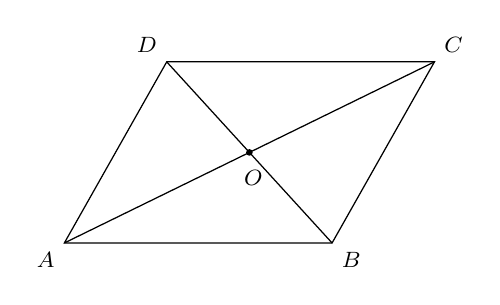
\begin{tikzpicture}[font=\footnotesize, line width=0.45pt, scale=1]
  \coordinate (A) at (0,0);
  \coordinate (B) at (3.4,0);
  \coordinate (C) at (4.7,2.3);
  \coordinate (D) at (1.3,2.3);
  \coordinate (O) at (2.35,1.15);
  \draw (A) -- (B) -- (C) -- (D) -- cycle;
  \draw (A) -- (C);
  \draw (B) -- (D);
  \fill (O) circle (1.2pt);
  \node[below left]  at (A) {$A$};
  \node[below right] at (B) {$B$};
  \node[above right] at (C) {$C$};
  \node[above left]  at (D) {$D$};
  \node[below]       at (2.40,1.05) {$O$};
\end{tikzpicture}
\end{center}
\nopagebreak[4]
\Needspace{4\baselineskip}
\textbf{解析}
\Needspace{5\baselineskip}
由平行四边形法则，
\nopagebreak[4]
\[\overrightarrow{AB}+\overrightarrow{AD}=\overrightarrow{AC}.\]
\Needspace{5\baselineskip}
又 $O$ 是平行四边形对角线的交点，即 $AC$ 的中点，故
\nopagebreak[4]
\[\overrightarrow{AC}=2\overrightarrow{AO}.\]
比较得 $\lambda=2$。

\gkanswer{答案：$2$。}

\end{answer}
\begin{answer}
\gksolhead{13}{}

\textbf{题目}：

已知函数 $f(x)=4x+\dfrac ax$（$x>0$，$a>0$）在 $x=3$ 时取得最小值，则 $a=$\gkblank{}。

\Needspace{4\baselineskip}
\textbf{解析}
\Needspace{5\baselineskip}
因 $x>0$，$a>0$，由基本不等式
\nopagebreak[4]
\[f(x)=4x+\frac ax\geqslant2\sqrt{4x\cdot\frac ax}=4\sqrt a,\]
等号当且仅当 $4x=\dfrac ax$，即 $x=\dfrac{\sqrt a}2$ 时成立。
\Needspace{5\baselineskip}
由题意最小值在 $x=3$ 处取得，故
\nopagebreak[4]
\[\frac{\sqrt a}2=3\implies\sqrt a=6\implies a=36.\]

\gkanswer{答案：$36$。}

\end{answer}
\begin{answer}
\gksolhead{14}{}

\textbf{题目}：

设 $\sin2\alpha=-\sin\alpha$，$\alpha\in\left(\dfrac\pi2,\pi\right)$，则 $\tan2\alpha$ 的值是\gkblank{}。

\Needspace{4\baselineskip}
\textbf{解析}
\Needspace{5\baselineskip}
由二倍角公式 $\sin2\alpha=2\sin\alpha\cos\alpha$，条件化为
\nopagebreak[4]
\[2\sin\alpha\cos\alpha=-\sin\alpha\implies\sin\alpha(2\cos\alpha+1)=0.\]
\Needspace{5\baselineskip}
因 $\alpha\in\left(\dfrac\pi2,\pi\right)$，$\sin\alpha>0$，故
\nopagebreak[4]
\[2\cos\alpha+1=0\implies\cos\alpha=-\frac12\implies\alpha=\frac{2\pi}3.\]
\Needspace{5\baselineskip}
于是 $2\alpha=\dfrac{4\pi}3$，
\nopagebreak[4]
\[\tan2\alpha=\tan\frac{4\pi}3=\tan\frac\pi3=\sqrt3.\]

\gkanswer{答案：$\sqrt3$。}

\end{answer}
\begin{answer}
\gksolhead{15}{}

\textbf{题目}：

在平面直角坐标系内，到点 $A(1,2)$，$B(1,5)$，$C(3,6)$，$D(7,-1)$ 的距离之和最小的点的坐标是\gkblank{}。

\Needspace{4\baselineskip}
\textbf{解析}
\Needspace{5\baselineskip}
设所求点为 $P$。把四个点两两配对：
\nopagebreak[4]
\[|PA|+|PC|\geqslant|AC|,\]
\Needspace{5\baselineskip}
等号当且仅当 $P$ 在线段 $AC$ 上；同理
\nopagebreak[4]
\[|PB|+|PD|\geqslant|BD|,\]
\Needspace{5\baselineskip}
等号当且仅当 $P$ 在线段 $BD$ 上。故
\nopagebreak[4]
\[|PA|+|PB|+|PC|+|PD|\geqslant|AC|+|BD|,\]
等号当且仅当 $P$ 同时在线段 $AC$ 与线段 $BD$ 上，即 $P$ 是两线段的交点。
\Needspace{5\baselineskip}
直线 $AC$ 过 $A(1,2)$，$C(3,6)$，斜率 $k=\dfrac{6-2}{3-1}=2$，方程为
\nopagebreak[4]
\[y-2=2(x-1)\implies y=2x.\]
\Needspace{5\baselineskip}
直线 $BD$ 过 $B(1,5)$，$D(7,-1)$，斜率 $k=\dfrac{-1-5}{7-1}=-1$，方程为
\nopagebreak[4]
\[y-5=-(x-1)\implies y=6-x.\]
联立 $2x=6-x$ 得 $x=2$，$y=4$。检验：$P(2,4)$ 在线段 $AC$ 上（$1\leqslant2\leqslant3$），也在线段 $BD$ 上（$1\leqslant2\leqslant7$），故等号可以取到。
所求点的坐标为 $(2,4)$。

\gkanswer{答案：$(2,4)$。}

\end{answer}
\begin{answer}
\gksolhead{16}{}

\textbf{题目}：

在等比数列 $\{a_n\}$ 中，$a_2-a_1=2$，且 $2a_2$ 为 $3a_1$ 和 $a_3$ 的等差中项，求数列 $\{a_n\}$ 的首项、公比及前 $n$ 项和。

\Needspace{4\baselineskip}
\textbf{解析}
设首项为 $a_1=a$，公比为 $q$，则 $a_2=aq$，$a_3=aq^2$。
\Needspace{5\baselineskip}
由 $a_2-a_1=2$ 得
\nopagebreak[4]
\[a(q-1)=2. \tag{1}\]
\Needspace{5\baselineskip}
由“$2a_2$ 为 $3a_1$ 和 $a_3$ 的等差中项”得
\nopagebreak[4]
\[2\cdot(2a_2)=3a_1+a_3\implies4aq=3a+aq^2,\]
\Needspace{5\baselineskip}
即
\nopagebreak[4]
\[a(q^2-4q+3)=0.\]
\Needspace{5\baselineskip}
因 $a(q-1)=2$，$a\neq0$，故
\nopagebreak[4]
\[q^2-4q+3=0\implies q=1\ \text{\text{或}}\ q=3.\]
\Needspace{5\baselineskip}
若 $q=1$，代入 (1) 得 $0=2$，矛盾；故
\nopagebreak[4]
\[q=3,\]
\Needspace{5\baselineskip}
再由 (1) 得
\nopagebreak[4]
\[a_1=a=\frac2{q-1}=1.\]
\Needspace{5\baselineskip}
于是
\nopagebreak[4]
\[a_n=3^{n-1},\qquad S_n=\frac{a_1(q^n-1)}{q-1}=\frac{3^n-1}{2}.\]
所以首项 $a_1=1$，公比 $q=3$，前 $n$ 项和 $S_n=\dfrac{3^n-1}2$。

\gkanswer{答案：首项 $a_1=1$，公比 $q=3$，前 $n$ 项和 $S_n=\dfrac{3^n-1}2$。}

\end{answer}
\begin{answer}
\gksolhead{17}{}

\textbf{题目}：

在 $\triangle ABC$ 中，角 $A$，$B$，$C$ 的对边分别为 $a$，$b$，$c$，且 $\cos(A-B)\cos B-\sin(A-B)\sin(A+C)=-\dfrac35$。
（1） 求 $\sin A$ 的值；
（2） 若 $a=4\sqrt2$，$b=5$，求向量 $\overrightarrow{BA}$ 在 $\overrightarrow{BC}$ 方向上的投影。

\Needspace{4\baselineskip}
\textbf{解析}
\Needspace{5\baselineskip}
\textbf{（1）} 因 $A+B+C=\pi$，故 $\sin(A+C)=\sin(\pi-B)=\sin B$。原条件化为
\nopagebreak[4]
\[\cos(A-B)\cos B-\sin(A-B)\sin B=-\frac35.\]
\Needspace{5\baselineskip}
由两角和的余弦公式，
\nopagebreak[4]
\[\cos(A-B)\cos B-\sin(A-B)\sin B=\cos\big[(A-B)+B\big]=\cos A,\]
\Needspace{5\baselineskip}
故
\nopagebreak[4]
\[\cos A=-\frac35.\]
\Needspace{5\baselineskip}
因 $A\in(0,\pi)$，$\sin A>0$，所以
\nopagebreak[4]
\[\sin A=\sqrt{1-\cos^2A}=\sqrt{1-\frac9{25}}=\frac45.\]
\Needspace{5\baselineskip}
\textbf{（2）} 由余弦定理 $a^2=b^2+c^2-2bc\cos A$，代入 $a=4\sqrt2$，$b=5$，$\cos A=-\dfrac35$：
\nopagebreak[4]
\[32=25+c^2-2\cdot5\cdot c\cdot\left(-\frac35\right)=25+c^2+6c,\]
\Needspace{5\baselineskip}
即
\nopagebreak[4]
\[c^2+6c-7=0\implies(c+7)(c-1)=0.\]
因 $c>0$，故 $c=1$。
\Needspace{5\baselineskip}
再由余弦定理求 $\cos B$：
\nopagebreak[4]
\[\cos B=\frac{a^2+c^2-b^2}{2ac}=\frac{32+1-25}{2\cdot4\sqrt2\cdot1}=\frac8{8\sqrt2}=\frac{\sqrt2}2.\]
\Needspace{5\baselineskip}
向量 $\overrightarrow{BA}$ 在 $\overrightarrow{BC}$ 方向上的投影为
\nopagebreak[4]
\[|\overrightarrow{BA}|\cos B=c\cos B=1\times\frac{\sqrt2}2=\frac{\sqrt2}2.\]

\gkanswer{答案（1）：$\dfrac45$。}

\gkanswer{答案（2）：$\dfrac{\sqrt2}{2}$。}

\end{answer}
\begin{answer}
\gksolhead{18}{}

\textbf{题目}：

某算法的程序框图如图所示，其中输入的变量 $x$ 在 $1,2,3,\cdots,24$ 这 $24$ 个整数中等可能随机产生。
\nopagebreak[4]
\begin{center}% 2013 四川卷文科第 18 题：输出 y 的值的程序框图。
\begin{tikzpicture}[font=\footnotesize, >=Stealth, line width=0.45pt,
  node distance=4.6mm,
  term/.style={draw, rounded corners=5pt, minimum height=1.8em, inner xsep=8pt},
  io/.style={draw, trapezium, trapezium left angle=72, trapezium right angle=108,
             minimum height=1.8em, inner xsep=7pt},
  box/.style={draw, minimum height=1.8em, inner xsep=6pt},
  dec/.style={draw, diamond, aspect=2.4, inner sep=1pt}]
  \node[term] (start) {开始};
  \node[io, below=5mm of start] (input) {输入 $x$};
  \node[dec, below=6mm of input] (even) {$x$ 为偶数?};
  \node[box, right=9mm of even] (y1) {$y=1$};
  \node[dec, below=9mm of even] (div) {$x$ 能被 3 整除?};
  \node[box, left=9mm of div] (y2) {$y=2$};
  \node[box, below=6mm of div] (y3) {$y=3$};
  \node[io, below=15mm of y3] (output) {输出 $y$};
  \node[term, below=5mm of output] (end) {结束};
  \draw[->] (start) -- (input);
  \draw[->] (input) -- (even);
  \draw[->] (even) -- node[above] {否} (y1);
  \draw[->] (even) -- node[right] {是} (div);
  \draw[->] (div) -- node[above] {否} (y2);
  \draw[->] (div) -- node[right] {是} (y3);
  \draw[->] (y1.south) |- (output.east);
  \draw[->] (y2.south) |- (output.west);
  \draw[->] (y3) -- (output);
  \draw[->] (output) -- (end);
\end{tikzpicture}
\end{center}
\nopagebreak[4]
（1） 分别求出按程序框图正确编程运行时输出 $y$ 的值为 $i$ 的概率 $P_i$（$i=1,2,3$）；
（2） 甲、乙两同学依据自己对程序框图的理解，各自编写程序重复运行 $n$ 次后，统计记录了输出 $y$ 的值为 $i$（$i=1,2,3$）的频数。以下是甲、乙所作频数统计表的部分数据。
甲的频数统计表（部分）：
\begin{center}
\begin{tabular}{llll}
\toprule
运行次数 $n$ & 输出 $y$ 为 $1$ 的频数 & 输出 $y$ 为 $2$ 的频数 & 输出 $y$ 为 $3$ 的频数 \\
\midrule
$30$ & $14$ & $6$ & $10$ \\
$\cdots$ & $\cdots$ & $\cdots$ & $\cdots$ \\
$2100$ & $1027$ & $376$ & $697$ \\
\bottomrule
\end{tabular}
\end{center}
乙的频数统计表（部分）：
\begin{center}
\begin{tabular}{llll}
\toprule
运行次数 $n$ & 输出 $y$ 为 $1$ 的频数 & 输出 $y$ 为 $2$ 的频数 & 输出 $y$ 为 $3$ 的频数 \\
\midrule
$30$ & $12$ & $11$ & $7$ \\
$\cdots$ & $\cdots$ & $\cdots$ & $\cdots$ \\
$2100$ & $1051$ & $696$ & $353$ \\
\bottomrule
\end{tabular}
\end{center}
当 $n=2100$ 时，根据表中的数据，分别写出甲、乙所编程序各自输出 $y$ 的值为 $i$（$i=1,2,3$）的频率（用分数表示），并判断两位同学中哪一位所编写程序符合算法要求的可能性较大。

\Needspace{4\baselineskip}
\textbf{解析}
\textbf{（1）} 由程序框图，$x$ 为奇数时输出 $y=1$；$x$ 为偶数时再看它能否被 $3$ 整除，不能整除输出 $y=2$，能整除输出 $y=3$。
在 $1,2,\cdots,24$ 中：
\begin{itemize}
\item 奇数共 $12$ 个，故 $P_1=\dfrac{12}{24}=\dfrac12$；
\item 偶数共 $12$ 个，其中能被 $3$ 整除的是 $6,12,18,24$ 共 $4$ 个，故不被 $3$ 整除的偶数有 $12-4=8$ 个，$P_2=\dfrac8{24}=\dfrac13$；
\item 能被 $3$ 整除的偶数有 $4$ 个，$P_3=\dfrac4{24}=\dfrac16$。
\end{itemize}
\Needspace{5\baselineskip}
\textbf{（2）} 当 $n=2100$ 时，甲所编程序输出 $y=1,2,3$ 的频率依次为
\nopagebreak[4]
\[\frac{1027}{2100}\approx0.4890,\qquad\frac{376}{2100}\approx0.1790,\qquad\frac{697}{2100}\approx0.3319;\]
\Needspace{5\baselineskip}
乙所编程序输出 $y=1,2,3$ 的频率依次为
\nopagebreak[4]
\[\frac{1051}{2100}\approx0.5005,\qquad\frac{696}{2100}\approx0.3314,\qquad\frac{353}{2100}\approx0.1681.\]
与算法要求的概率 $\dfrac12\approx0.5$，$\dfrac13\approx0.3333$，$\dfrac16\approx0.1667$ 比较：
甲的三个频率与 $\dfrac12$，$\dfrac13$，$\dfrac16$ 的偏差分别约为 $0.011$，$0.154$，$0.165$；
乙的偏差分别约为 $0.0005$，$0.0019$，$0.0014$。
乙的三组频率都稳定在相应概率附近，而甲的第二、三组频率与 $\dfrac13$，$\dfrac16$ 相差很远（甲把“偶数且不被 $3$ 整除”与“偶数且被 $3$ 整除”两类混淆了），故乙所编写的程序符合算法要求的可能性较大。

\gkanswer{答案（1）：$P_1=\dfrac12$，$P_2=\dfrac13$，$P_3=\dfrac16$。}

\gkanswer{答案（2）：甲为 $\dfrac{1027}{2100}$，$\dfrac{376}{2100}$，$\dfrac{697}{2100}$；乙为 $\dfrac{1051}{2100}$，$\dfrac{696}{2100}$，$\dfrac{353}{2100}$；乙所编写程序符合算法要求的可能性较大。}

\end{answer}
\begin{answer}
\gksolhead{19}{}

\textbf{题目}：

如图，在三棱柱 $ABC-A_1B_1C_1$ 中，侧棱 $AA_1\perp$ 底面 $ABC$，$AB=AC=2AA_1=2$，$\angle BAC=120^\circ$，$D$，$D_1$ 分别是线段 $BC$，$B_1C_1$ 的中点，点 $P$ 是线段 $AD$ 上异于端点的点。
\nopagebreak[4]
\begin{center}% 2013 四川卷文科第 19 题：三棱柱 ABC-A1B1C1，D、D1 分别为 BC、B1C1 的中点，P 在 AD 上。
\begin{tikzpicture}[font=\footnotesize, line width=0.45pt, scale=1]
  \coordinate (C)  at (0.80,3.40);
  \coordinate (A)  at (2.60,2.00);
  \coordinate (B)  at (5.60,2.00);
  \coordinate (C1) at (0.80,1.60);
  \coordinate (A1) at (2.60,0.20);
  \coordinate (B1) at (5.60,0.20);
  \coordinate (D)  at (3.20,2.70);
  \coordinate (D1) at (3.20,0.90);
  \coordinate (P)  at (2.87,2.315);
  % 顶面三角形
  \draw (A) -- (B) -- (C) -- cycle;
  % 可见的侧棱与底面棱
  \draw (A) -- (A1);
  \draw (B) -- (B1);
  \draw (C) -- (C1);
  \draw (A1) -- (B1);
  % 平面 A1BC 的辅助线
  \draw (A1) -- (C);
  \draw (A1) -- (B);
  % 被遮挡的棱
  \draw[dashed] (C1) -- (A1);
  \draw[dashed] (C1) -- (B1);
  \draw[dashed] (D)  -- (D1);
  % 点与标注
  \fill (P) circle (1.4pt);
  \node[above left]  at (C)  {$C$};
  \node[below left]  at (2.48,1.86) {$A$};
  \node[right]       at (B)  {$B$};
  \node[left=3pt]    at (C1) {$C_1$};
  \node[below left]  at (A1) {$A_1$};
  \node[below right=1pt] at (B1) {$B_1$};
  \node[above left]  at (D)  {$D$};
  \node[right]       at ($(D1)+(0.10,0)$) {$D_1$};
  \node[left]        at (P)  {$P$};
\end{tikzpicture}
\end{center}
\nopagebreak[4]
（1） 在平面 $ABC$ 内，试作出过点 $P$ 与平面 $A_1BC$ 平行的直线 $l$，请说明理由，并证明直线 $l\perp$ 平面 $ADD_1A_1$；
（2） 设（1）中的直线 $l$ 交 $AC$ 于点 $Q$，求三棱锥 $A_1-QC_1D$ 的体积。
（锥体体积公式：$V=\dfrac13Sh$，其中 $S$ 为底面面积，$h$ 为高）

\Needspace{4\baselineskip}
\textbf{解析}
\textbf{（1）} 因为 $l\subset$ 平面 $ABC$，平面 $A_1BC\cap$ 平面 $ABC=BC$，且 $l\parallel$ 平面 $A_1BC$，由线面平行的性质定理得 $l\parallel BC$。
作法：在平面 $ABC$ 内过点 $P$ 作 $BC$ 的平行线，该直线与 $AB$、$AC$ 都相交，即为所求的直线 $l$。
证明 $l\perp$ 平面 $ADD_1A_1$：
\Needspace{5\baselineskip}
因 $AB=AC$ 且 $D$ 为 $BC$ 的中点，故 $AD\perp BC$；又 $l\parallel BC$，所以
\nopagebreak[4]
\[l\perp AD.\]
\Needspace{5\baselineskip}
因 $AA_1\perp$ 平面 $ABC$，$l\subset$ 平面 $ABC$，故
\nopagebreak[4]
\[l\perp AA_1.\]
\Needspace{5\baselineskip}
而 $AD\cap AA_1=A$，$AD$，$AA_1\subset$ 平面 $ADD_1A_1$，所以
\nopagebreak[4]
\[l\perp\text{\text{平面}}\ ADD_1A_1.\]
\textbf{（2）} 由 $AB=AC=2AA_1=2$ 得 $AB=AC=2$，$AA_1=1$。
\Needspace{5\baselineskip}
以 $A$ 为原点，在平面 $ABC$ 内以 $AB$ 为 $x$ 轴、以过 $A$ 且垂直于 $AB$ 的方向为 $y$ 轴、以 $\overrightarrow{AA_1}$ 的方向为 $z$ 轴，建立空间直角坐标系。由 $\angle BAC=120^\circ$ 得
\nopagebreak[4]
\[A(0,0,0),\quad B(2,0,0),\quad C\left(-1,\sqrt3,0\right),\quad A_1(0,0,1),\]
\Needspace{5\baselineskip}
从而
\nopagebreak[4]
\[C_1\left(-1,\sqrt3,1\right),\quad D\left(\frac12,\frac{\sqrt3}2,0\right).\]
\Needspace{5\baselineskip}
设 $\dfrac{AQ}{AC}=\dfrac{AP}{AD}=t$（$0<t<1$），由 $l\parallel BC$ 知 $\triangle APQ\sim\triangle ADC$，故
\nopagebreak[4]
\[Q\left(-t,\sqrt3t,0\right).\]
\Needspace{5\baselineskip}
于是
\nopagebreak[4]
\[\overrightarrow{A_1Q}=\left(-t,\sqrt3t,-1\right),\quad\overrightarrow{A_1C_1}=\left(-1,\sqrt3,0\right),\quad\overrightarrow{A_1D}=\left(\frac12,\frac{\sqrt3}2,-1\right).\]
\Needspace{5\baselineskip}
三棱锥 $A_1-QC_1D$ 的体积为
\nopagebreak[4]
\[V=\frac16\left|\begin{vmatrix}-t&\sqrt3t&-1\\ -1&\sqrt3&0\\ \frac12&\frac{\sqrt3}2&-1\end{vmatrix}\right|.\]
\Needspace{5\baselineskip}
按第一行展开：
\nopagebreak[4]
\[\begin{aligned}
&\ (-t)\left[\sqrt3\cdot(-1)-0\cdot\frac{\sqrt3}2\right]-\sqrt3t\left[(-1)\cdot(-1)-0\cdot\frac12\right]+(-1)\left[(-1)\cdot\frac{\sqrt3}2-\sqrt3\cdot\frac12\right]\\
=&\ (-t)(-\sqrt3)-\sqrt3t\cdot1+(-1)\left(-\frac{\sqrt3}2-\frac{\sqrt3}2\right)=\sqrt3t-\sqrt3t+\sqrt3=\sqrt3.
\end{aligned}\]
\Needspace{5\baselineskip}
故
\nopagebreak[4]
\[V=\frac16\times\sqrt3=\frac{\sqrt3}6,\]
与点 $P$ 在 $AD$ 上的位置无关。

\gkanswer{答案（1）：过 $P$ 作 $BC$ 的平行线即为 $l$；作图和证明见解析。}

\gkanswer{答案（2）：$\dfrac{\sqrt3}{6}$。}

\end{answer}
\begin{answer}
\gksolhead{20}{}

\textbf{题目}：

已知圆 $C$ 的方程为 $x^2+(y-4)^2=4$，点 $O$ 是坐标原点，直线 $l$：$y=kx$ 与圆 $C$ 交于 $M$，$N$ 两点。
（1） 求 $k$ 的取值范围；
（2） 设 $Q(m,n)$ 是线段 $MN$ 上的点，且 $\dfrac2{|OQ|^2}=\dfrac1{|OM|^2}+\dfrac1{|ON|^2}$，请将 $n$ 表示为 $m$ 的函数。

\Needspace{4\baselineskip}
\textbf{解析}
\textbf{（1）} 圆 $C$：$x^2+(y-4)^2=4$ 的圆心为 $(0,4)$，半径为 $2$。
\Needspace{5\baselineskip}
直线 $l$：$y=kx$ 即 $kx-y=0$。$l$ 与圆交于两点，等价于圆心到 $l$ 的距离小于半径：
\nopagebreak[4]
\[\frac{|k\cdot0-4|}{\sqrt{k^2+1}}<2\implies\frac4{\sqrt{k^2+1}}<2\implies\sqrt{k^2+1}>2\implies k^2>3.\]
故 $k$ 的取值范围是 $k<-\sqrt3$ 或 $k>\sqrt3$。
\Needspace{5\baselineskip}
\textbf{（2）} 把 $y=kx$ 代入圆的方程：
\nopagebreak[4]
\[x^2+(kx-4)^2=4\implies\left(1+k^2\right)x^2-8kx+12=0.\]
\Needspace{5\baselineskip}
设 $M(x_1,y_1)$，$N(x_2,y_2)$，则
\nopagebreak[4]
\[x_1+x_2=\frac{8k}{1+k^2},\qquad x_1x_2=\frac{12}{1+k^2}.\]
\Needspace{5\baselineskip}
因 $y_i=kx_i$，故
\nopagebreak[4]
\[|OM|^2=\left(1+k^2\right)x_1^2,\qquad|ON|^2=\left(1+k^2\right)x_2^2,\]
\Needspace{5\baselineskip}
从而
\nopagebreak[4]
\[\frac1{|OM|^2}+\frac1{|ON|^2}=\frac1{1+k^2}\left(\frac1{x_1^2}+\frac1{x_2^2}\right)=\frac1{1+k^2}\cdot\frac{(x_1+x_2)^2-2x_1x_2}{(x_1x_2)^2}.\]
\Needspace{5\baselineskip}
其中
\nopagebreak[4]
\[(x_1+x_2)^2-2x_1x_2=\frac{64k^2}{(1+k^2)^2}-\frac{24}{1+k^2}=\frac{40k^2-24}{(1+k^2)^2},\qquad(x_1x_2)^2=\frac{144}{(1+k^2)^2},\]
\Needspace{5\baselineskip}
代入得
\nopagebreak[4]
\[\frac1{|OM|^2}+\frac1{|ON|^2}=\frac{40k^2-24}{144(1+k^2)}=\frac{5k^2-3}{18(1+k^2)}.\]
\Needspace{5\baselineskip}
点 $Q(m,n)$ 在直线 $l$ 上，故 $n=km$，$|OQ|^2=(1+k^2)m^2$，于是条件
\nopagebreak[4]
\[\frac2{|OQ|^2}=\frac1{|OM|^2}+\frac1{|ON|^2}\]
\Needspace{5\baselineskip}
化为
\nopagebreak[4]
\[\frac2{(1+k^2)m^2}=\frac{5k^2-3}{18(1+k^2)}\implies m^2\left(5k^2-3\right)=36.\]
\Needspace{5\baselineskip}
把 $k=\dfrac nm$ 代入：
\nopagebreak[4]
\[5n^2-3m^2=36\implies n^2=\frac{3m^2+36}5.\]
\Needspace{5\baselineskip}
因圆 $C$ 上的点满足 $y\in[2,6]$，故线段 $MN$ 上的点 $Q$ 恒有 $n>0$，所以
\nopagebreak[4]
\[n=\sqrt{\frac{3m^2+36}5}=\frac{\sqrt{15m^2+180}}5.\]
由 $m^2=\dfrac{36}{5k^2-3}$ 及 $k^2>3$ 得 $0<m^2<3$，即 $-\sqrt3<m<\sqrt3$ 且 $m\neq0$。
\Needspace{5\baselineskip}
所求函数为
\nopagebreak[4]
\[n=\frac{\sqrt{15m^2+180}}5\quad\left(-\sqrt3<m<\sqrt3,\ m\neq0\right).\]

\gkanswer{答案（1）：$k<-\sqrt3$ 或 $k>\sqrt3$。}

\gkanswer{答案（2）：$n=\dfrac{\sqrt{15m^2+180}}5$（$-\sqrt3<m<\sqrt3$ 且 $m\neq0$）。}

\end{answer}
\begin{answer}
\gksolhead{21}{}

\textbf{题目}：

已知函数 $f(x)=\begin{cases}x^2+2x+a,&x<0,\\[2pt] \ln x,&x>0,\end{cases}$ 其中 $a$ 是实数。设 $A(x_1,f(x_1))$，$B(x_2,f(x_2))$ 为该函数图象上的两点，且 $x_1<x_2$。
（1） 指出函数 $f(x)$ 的单调区间；
（2） 若函数 $f(x)$ 的图象在点 $A$，$B$ 处的切线互相垂直，且 $x_2<0$，证明：$x_2-x_1\geqslant1$；
（3） 若函数 $f(x)$ 的图象在点 $A$，$B$ 处的切线重合，求 $a$ 的取值范围。

\Needspace{4\baselineskip}
\textbf{解析}
\textbf{（1）} 当 $x<0$ 时，$f'(x)=2x+2$；当 $x>0$ 时，$f'(x)=\dfrac1x>0$。
由 $2x+2<0$ 得 $x<-1$；由 $2x+2>0$ 得 $-1<x<0$。
故 $f(x)$ 的单调递减区间为 $(-\infty,-1)$，单调递增区间为 $(-1,0)$ 和 $(0,+\infty)$。
\textbf{（2）} 由 $x_2<0$ 及 $x_1<x_2$ 知 $x_1<x_2<0$，两点都在抛物线弧上，$f'(x_1)=2x_1+2$，$f'(x_2)=2x_2+2$。
\Needspace{5\baselineskip}
两切线互相垂直，故
\nopagebreak[4]
\[(2x_1+2)(2x_2+2)=-1.\]
\Needspace{5\baselineskip}
令 $u_1=2x_1+2$，$u_2=2x_2+2$，则 $u_1<u_2<2$ 且 $u_1u_2=-1<0$，故
\nopagebreak[4]
\[u_1<0<u_2.\]
\Needspace{5\baselineskip}
于是
\nopagebreak[4]
\[x_2-x_1=\frac{u_2-u_1}2=\frac{u_2+\frac1{u_2}}2\geqslant\frac{2\sqrt{u_2\cdot\frac1{u_2}}}2=1,\]
等号当且仅当 $u_2=1$（即 $x_2=-\dfrac12$，$x_1=-\dfrac32$）时成立。
所以 $x_2-x_1\geqslant1$。
\Needspace{5\baselineskip}
\textbf{（3）} 先说明两切点必分居两段。若 $x_1<x_2<0$，两点都在抛物线上，切线斜率 $2x+2$ 严格递增，两条切线斜率不等，不可能重合；若 $0<x_1<x_2$，切线斜率 $\dfrac1x$ 严格递减，也不可能重合。故
\nopagebreak[4]
\[x_1<0<x_2.\]
切线重合须斜率相等、截距相等。
\Needspace{5\baselineskip}
斜率：$f'(x_1)=2x_1+2$，$f'(x_2)=\dfrac1{x_2}$，故
\nopagebreak[4]
\[2x_1+2=\frac1{x_2}. \tag{1}\]
\Needspace{5\baselineskip}
由 $x_1<0$ 及 (1) 得 $\dfrac1{x_2}<2$，结合 $x_2>0$ 得
\nopagebreak[4]
\[x_2>\frac12,\qquad x_1=\frac1{2x_2}-1.\]
\Needspace{5\baselineskip}
截距：点 $A$ 处切线为
\nopagebreak[4]
\[y=(2x_1+2)(x-x_1)+x_1^2+2x_1+a=(2x_1+2)x+\left(a-x_1^2\right),\]
\Needspace{5\baselineskip}
点 $B$ 处切线为
\nopagebreak[4]
\[y=\frac1{x_2}(x-x_2)+\ln x_2=\frac1{x_2}x+\left(\ln x_2-1\right).\]
\Needspace{5\baselineskip}
由截距相等得
\nopagebreak[4]
\[a=x_1^2+\ln x_2-1.\]
\Needspace{5\baselineskip}
令 $t=x_2>\dfrac12$，代入 $x_1=\dfrac1{2t}-1$：
\nopagebreak[4]
\[a=\left(\frac1{2t}-1\right)^2+\ln t-1=\frac1{4t^2}-\frac1t+\ln t=:h(t).\]
\Needspace{5\baselineskip}
求导：
\nopagebreak[4]
\[h'(t)=-\frac1{2t^3}+\frac1{t^2}+\frac1t=\frac{2t^2+2t-1}{2t^3}.\]
当 $t>\dfrac12$ 时，$2t^2+2t-1>2\cdot\dfrac14+2\cdot\dfrac12-1=\dfrac12>0$，故 $h'(t)>0$，$h$ 在 $\left(\dfrac12,+\infty\right)$ 上严格递增。
\Needspace{5\baselineskip}
又
\nopagebreak[4]
\[h\left(\frac12\right)=1-2+\ln\frac12=-1-\ln2,\]
且 $t\to+\infty$ 时 $h(t)\to+\infty$，故 $h$ 的值域为 $\left(-1-\ln2,+\infty\right)$。
\Needspace{5\baselineskip}
所以 $a$ 的取值范围是
\nopagebreak[4]
\[a\in\left(-1-\ln2,+\infty\right).\]

\gkanswer{答案（1）：单调递减区间为 $(-\infty,-1)$，单调递增区间为 $(-1,0)$ 和 $(0,+\infty)$。}

\gkanswer{答案（2）：证明见解析。}

\gkanswer{答案（3）：$a\in(-1-\ln2,+\infty)$。}

\end{answer}